\section{System description}
\label{sec:system_description}

\subsection{General overview}
\label{subsec:overview}

Offshore platforms are large structures with facilities to extract and process petroleum from subsea reservoirs. Petroleum is processed in a processing plant using power (and often also heat) that is produced in a utility plant. The power is produced by gas turbines fuelled with a fraction of produced gas, or, alternatively, heavy oil or diesel. A heating demand is either met by using fuel gas burners, electric heaters or by indirect waste heat recovery. 

In this work we distinguish between three different control volumes: the processing plant, the utility plant and the overall plant (which is the combination of the processing plant and the utility plant). The drilling- and accomodation parts are not included in the study. The control volumes with the in- and outgoing material- and energy streams are shown schematically in Figure~\ref{fig:control_volume}. 

\begin{figure*}[htbp]
	\centering
	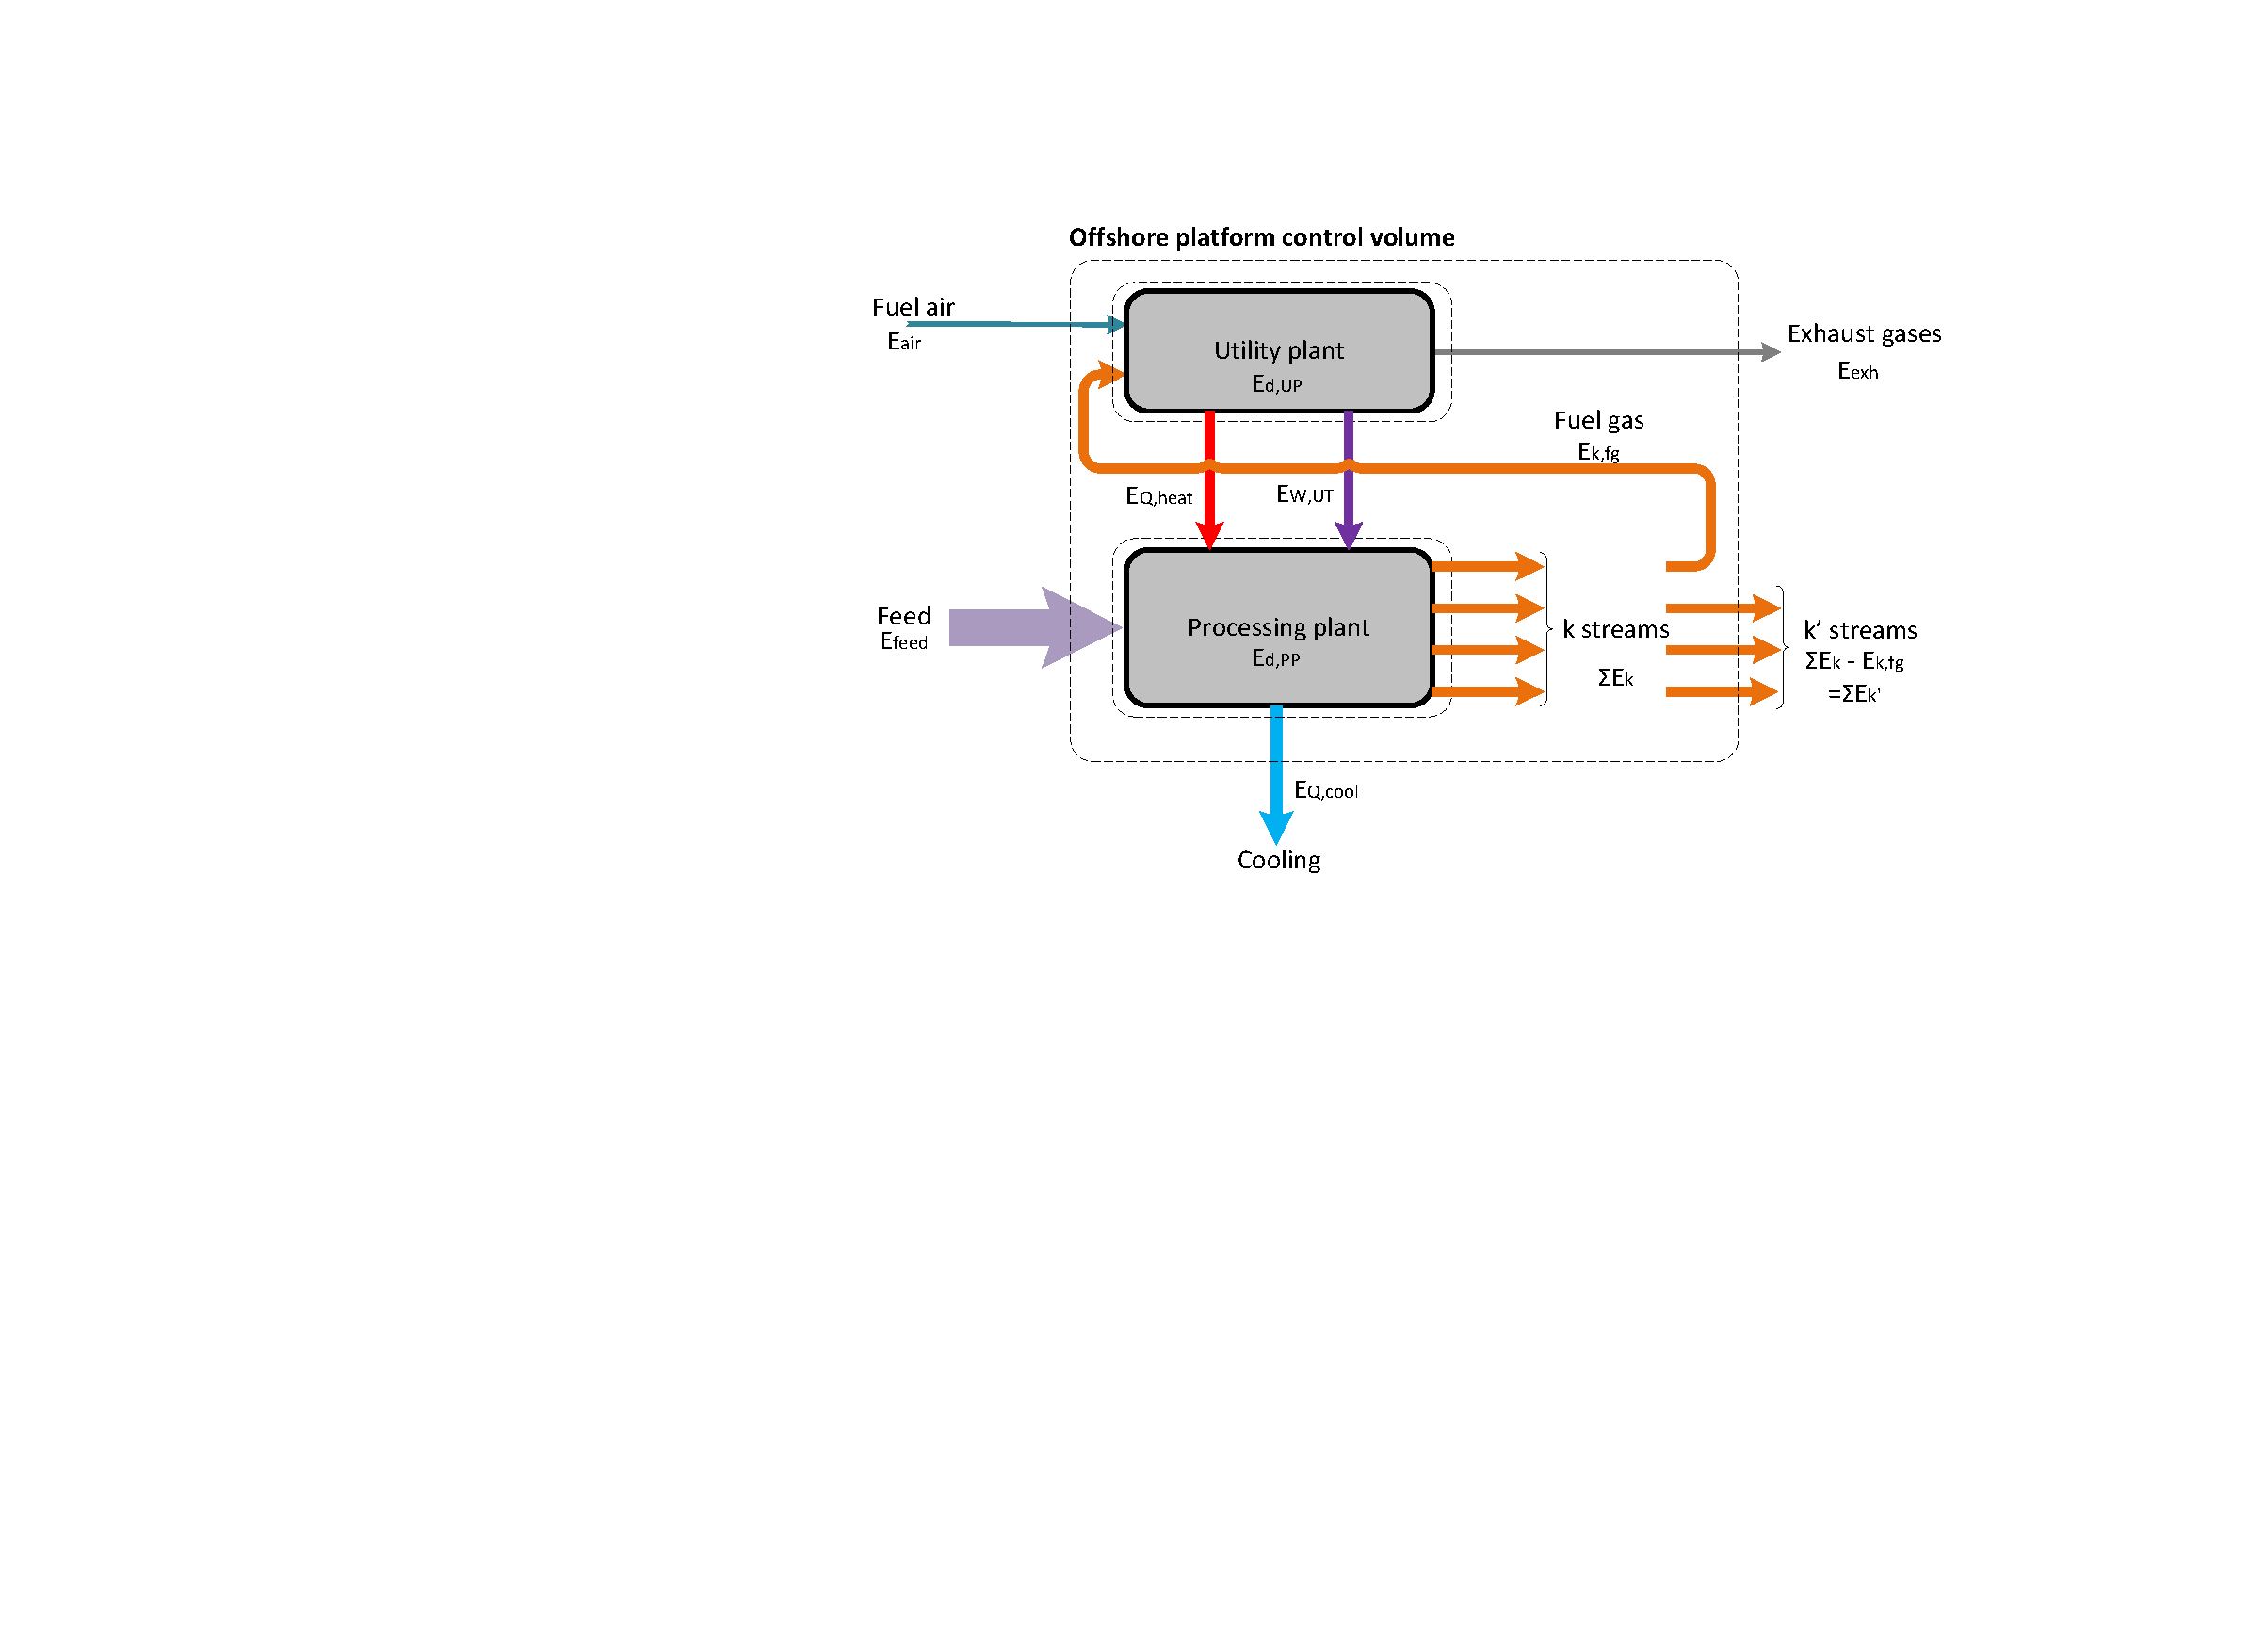
\includegraphics[width=0.75\textwidth]{control_volume.pdf}
	\caption{Control volume of oil and gas offshore facilities. \textbf{Ok to move this figure here? Maybe remove the exergy notation? But then we have to show it later again, so I don't know... What do you think, TV? Mark also that some output streams can be useful and some lost, ku and kw? Maybe best to have a very simple version here, and a version with notation in the section about efficiency?}}
	\label{fig:control_volume}
\end{figure*}

Petroleum is a complex multiphase mixture: it contains a large spectrum of chemical compounds, from light hydrocarbons in gaseous form (e.g. methane) to heavy ones in liquid phase (e.g. naphtenes and cycloalkanes) and is extracted along with subsurface water. The aim of the processing plant is to separate efficiently the different phases to satisfy the different process and export constraints, and to maximise the hydrocarbon production. Crude oil consists mostly of medium- to heavy hydrocarbons in liquid form, while natural gas mostly consists of light-weight alkanes. Differences across offshore platforms can be summarised as follows \cite{Bothamley2004,Energistyrelsen2011,NorwegianMinistryofPetroleumandEnergy2012,JonesDavidS.J.Stan;Pujado2006,Manning1991,Plisga2004,Abdel-AalH.K.;AggourMohamed;Fahim2003,VikEilanArctander;Dinning2009}: 

\begin{itemize}
	\item reservoir characteristics (e.g. initial temperature and pressure);
	\item fluid properties (e.g. chemical composition, gas- and water-to-oil (GOR and WOR)\nomenclature[A]{GOR}{Gas-to-Oil Ratio}\nomenclature[A]{WOR}{Water-to-Oil Ratio} ratios);
	\item product requirements (e.g. export pressure and temperature, chemical purity);
	\item operating strategies (e.g. oil and gas recovery, gas treatment, condensate export).
\end{itemize}
These differences induce variations in temperatures, pressures and flow rates throughout the system as well as in demands for compression, heating, cooling, dehydration, desalting and sweetening. The structural design of the processing plant stays nevertheless similar and a schematic overview is given in Figure~\ref{fig:processing_plant}.

\begin{figure*}[htbp]
	\centering
	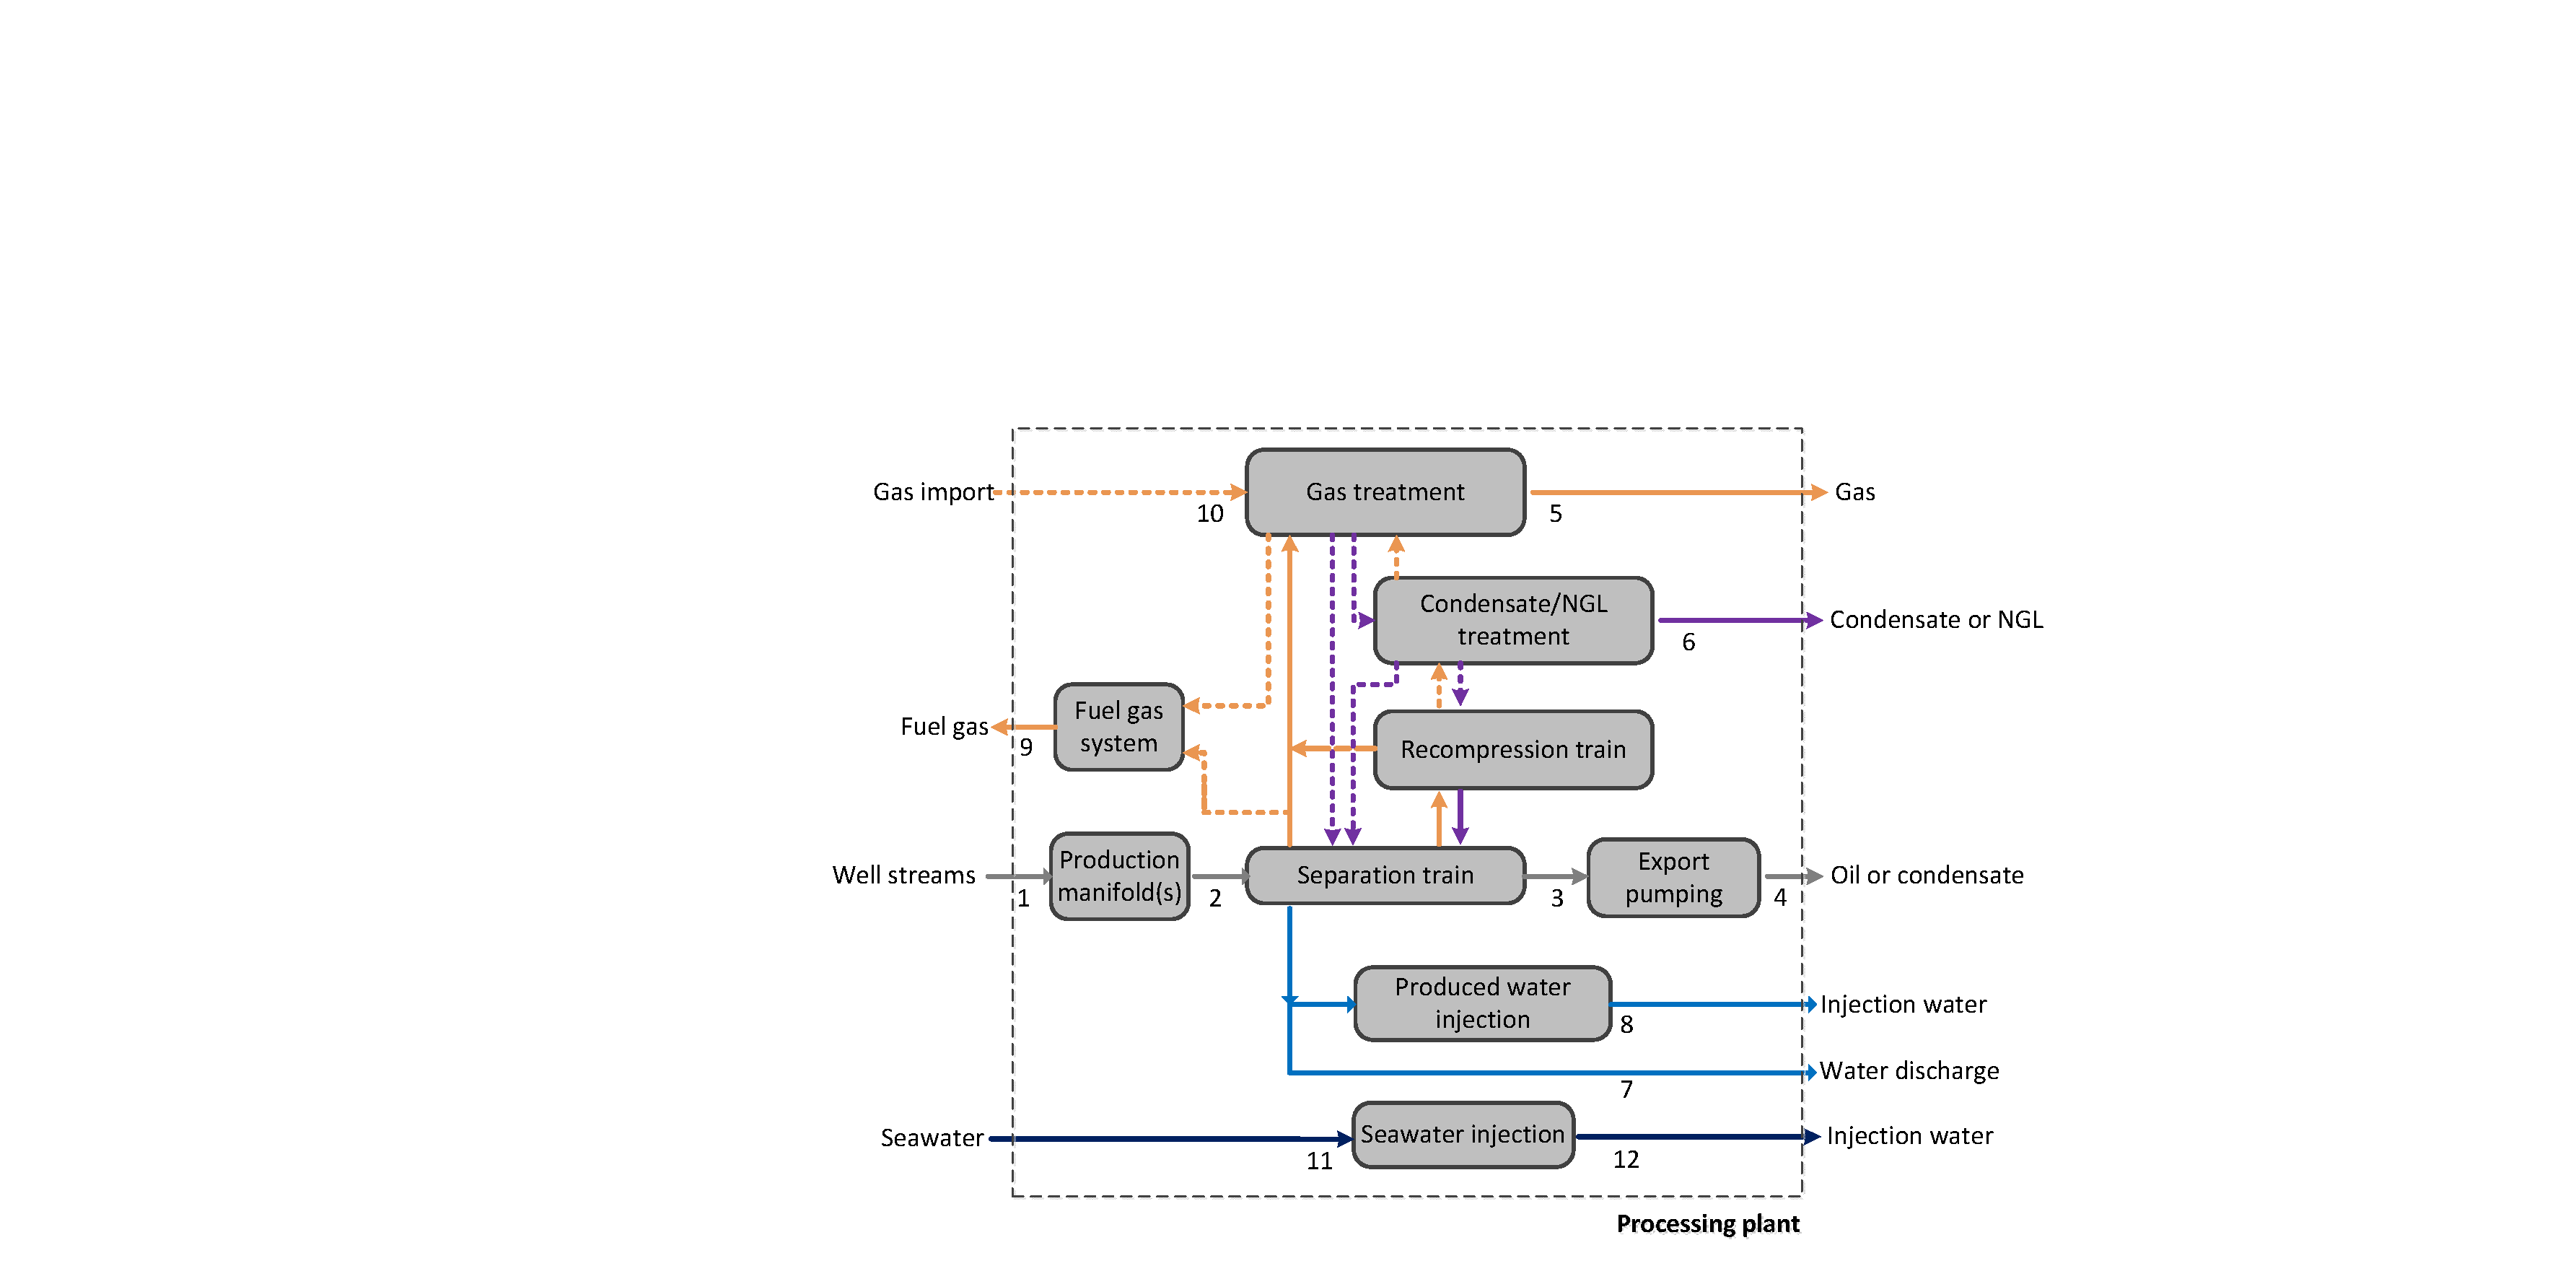
\includegraphics[width=0.75\textwidth]{general_process_overview.pdf}
	\caption{General overview of the processing plant}
	\label{fig:processing_plant}
\end{figure*}

In the processing plant oil, gas and water enter one or several production manifolds in which the well-fluid streams are mixed and the pressure reduced to ease separation between the liquid and gaseous phases. The well-fluid streams are fed into a separation system where oil, gas and water are separated by gravity in one to several stages, with throttling in between. Crude oil leaving the separation train enters a treatment and export pumping section. Gas leaving the separation and oil pumping steps enters the recompression train. It is cooled, sent to a scrubber where condensate and water droplets are removed, and recompressed to the pressure of the previous separation stage. It is then sent to the gas treatment train, where it is purified and possibly dehydrated by triethylene glycol (TEG)\nomenclature[A]{TEG}{Triethylene Glycol}. Gas may be compressed for export to the shore, lift or injection. 

Condensate removed from the recompression and gas treatment trains is (i) either sent back to the separation train and mixed with crude oil or (ii) processed apart in a condensate treatment section. Produced water enters a wastewater handling train, in which suspended particulates and dissolved hydrocarbons are removed. It is then discharged into the sea or enters an injection train where it is further cleaned and pumped to a high pressure level. In parallel, seawater may be processed onsite for further injection into the reservoir for enhanced oil recovery. 
	
The cooling demand is satisfied by using a direct cooling medium, e.g. seawater or air, or an indirect one, e.g. a glycol/water mixture. Heat exchanger networks between the several streams flowing through the system may also be integrated to promote heat integration.

Processes such as condensate treatment and natural gas liquid recovery are uncommon offshore, with only a few applications worldwide. Oil and gas treatment is generally limited to gas dehydration in the North Sea, whereas it also includes oil desalting and gas sweetening in the Gulf of Mexico. Further details on oil and gas processing are given in \cite{Manning1991a} and more specific information on North Sea platforms are given in Refs. \cite{Bothamley2004,Nguyen2013}.

\subsection{Case studies}
\label{subsec:specific}

The four oil and gas platforms investigated within this study are located in the North Sea region and present specific design characteristics (\emph{Figure \ref{fig:processing_plant}} and \emph{Table \ref{tab:platform_characteristics}}). 

\begin{table*}[htbp]
\scriptsize
  \centering
  \caption{Comparison of the four offshore facilities discussed in this study}
    \begin{tabular}{lllll}
    \toprule
    \textbf{Platform} & A     & B     & C     & D \\
    \midrule
    \textbf{System characteristics} &       &       &       &  \\
    Age (years) & 20    & 10    & 10    & 20 \\
    Gas-to-oil ratio & increasing & increasing & increasing & decreasing \\
    \textbf{} &       &       &       &  \\
    \textbf{System products} &       &       &       &  \\
    Oil   & export & none  & export & export \\
    Gas   & fuel  & fuel  & fuel  & fuel \\
          & injection & export & injection & export \\
          &       &       & import &  \\
          &       &       & lift  &  \\
    Condensate & export & export & export & export \\
          & (mixed with oil) &       & (mixed with oil) & (mixed with gas) \\
    Produced water & discharge & discharge & discharge & discharge \\
          &       &       &       & injection \\
    Seawater & cooling & cooling & cooling & cooling \\
          &       &       &       & injection \\
          &       &       &       & (complement) \\
    \textbf{Additional processes} &       &       &       &  \\
    Dehydration & n     & n     & n     & y \\
    Condensate treatment & n     & n     & n     & y \\
    Water injection  & n     & n     & n     & y \\
    \bottomrule
    \end{tabular}%
  \label{tab:platform_characteristics}%
\end{table*}%

%\begin{enumerate}
%	\item Platform A has been in operation for about 20 years and produces \emph{crude oil} and \emph{associated gas}. Crude oil is exported to another platform via pipelines for further export to the shore. Associated gas is compressed and injected into the reservoir for pressure maintenance, along with injection water produced at another platform. Produced water is treated and rejected to the sea. At the moment, oil production decreases while oil production increases.
%	\item Platform B has been in operation for about 10 years and produces \emph{gas} and \emph{condensate}. Produced gas is directly exported to the shore and recovered condensate is sent onshore via pipelines. Produced water is cleaned and discharged into a separate reservoir.
%	\item Platform C has been in operation for about 10 years and produces \emph{crude oil} and \emph{associated gas}. Gas is used for both gas lift, to ease the reservoir fluid extraction, and for gas injection, to sustain a high pressure. Produced water is also discharged into a separate reservoir. Heat integration is achieved by heat exchanges between the crude oil streams in the separation and pumping sections.
%	\item Platform D has been in operation for about 20 years and produces \emph{crude oil}, \emph{gas} and \emph{condensate}. Crude oil is stored at the bottom of the facility in oil cells and is exported onshore twice a week via shuttle tanks. Gas and condensate are dehydrated: only small amounts of gas are exported, the major fraction is used for gas lift and power generation onsite. Produced water is treated and injected back into the reservoir for pressure maintenance, alongside with seawater. Waste heat from two of the onsite gas turbines is partly recovered and used for enhancing glycol regeneration in the dehydration process and crude oil separation in the separation subsystem. 
%\end{enumerate}



These four platforms, although similar in terms of structural design, present significant differences in well-fluid processing and in operating conditions: 

\begin{itemize}
	\item The gas-to-oil ratio is either increasing (e.g. platforms A and B), meaning that the gas treatment train is run at full-design conditions or decreasing (e.g. platforms C and D), meaning that this subsystem is run in off-design conditions, and that anti-surge recycling is practiced to protect the compressors.
	\item Platforms processing heavy and viscous crude oil (e.g. platform C) or with a high propane content (e.g. platform D) require heating in the separation train to enhance vapour-liquid separation and to meet the export specifications.
	\item The pressure at the final stage of the separation train ($p_3$) is constrained by the maximum allowable vapour pressure of the crude oil/condensate in the pipelines and shuffle tankers, and is below 3 bar for all platforms.
	\item The pressure of the produced oil/condensate at the outlet of the pumping section ($p_4$) is either higher (e.g. platform C) or lower (e.g. platforms A, B and D) than at the outlet of the production manifold ($p_2$).
	\item The pressure at the outlet of the gas treatment section ($p_5$) is either higher (e.g. platforms A, C and D) or lower (e.g. platform B) than at the inlet of the separation system ($p_2$). There is a need for gas compression in three of the four platforms. 
\end{itemize} 

For more details about the processes taking place on each of these platforms, the reader is referred to two previous works conducted by the same authors \cite{Voldsund2013,Voldsund2013b}. 

\subsection{Modelling and simulation}

The process simulations were carried out with Aspen HYSYS\textsuperscript{\tiny\textregistered} \cite{Guide2004} and Aspen Plus\textsuperscript{\tiny\textregistered} version 7.2\ \cite{Technology1999}, with the exception of the glycol dehydration system. Simulations of the production manifolds, petroleum separation, oil pumping, gas recompression and flaring were based on the Peng-Robinson equation of state (EOS)\nomenclature[A]{EOS}{Equation of State} \cite{Peng1976}. The water purification and injection processes were simulated based on the Non-Random Two Liquid (NRTL) model \cite{Renon1968} and the dehydration process on the Schwartzentruber-Renon EOS \cite{Schwartzentruber1989a,Schwartzentruber1989b}. Power generation was simulated by using the in-house tool DNA (Dynamic Network Analysis), which is a program developed at the Technical University of Denmark \cite{Elmegaard2005}. 

